\documentclass[tikz,border=8pt]{standalone}
% Shared look for every TikZ diagram. Load with \input{../../tools/tikz-style.tex}
\usepackage[T1]{fontenc}
\usepackage{lmodern}
\renewcommand{\sfdefault}{lmr}  % diagrams use the same serif as the text
\usetikzlibrary{arrows.meta, positioning, shapes.geometric, calc, fit, backgrounds}
\definecolor{cblue}{HTML}{4C78A8}
\definecolor{corange}{HTML}{F58518}
\definecolor{cgreen}{HTML}{54A24B}
\definecolor{cred}{HTML}{E45756}
\definecolor{cpurple}{HTML}{B279A2}
\definecolor{cgrey}{HTML}{6B6B6B}
\tikzset{
  every picture/.style={font=\sffamily, line width=1.2pt},
  box/.style={draw=#1, fill=#1!12, rounded corners=4pt, align=center, inner sep=7pt, minimum height=1.1cm},
  box/.default=cgrey,
  arrow/.style={-{Stealth[length=3mm]}, draw=cgrey, line width=1.4pt},
  title/.style={font=\sffamily\bfseries\Large},
  note/.style={font=\sffamily\small, text=cgrey, align=center},
}
\AtBeginDocument{\hyphenpenalty=10000 \exhyphenpenalty=10000}

\begin{document}
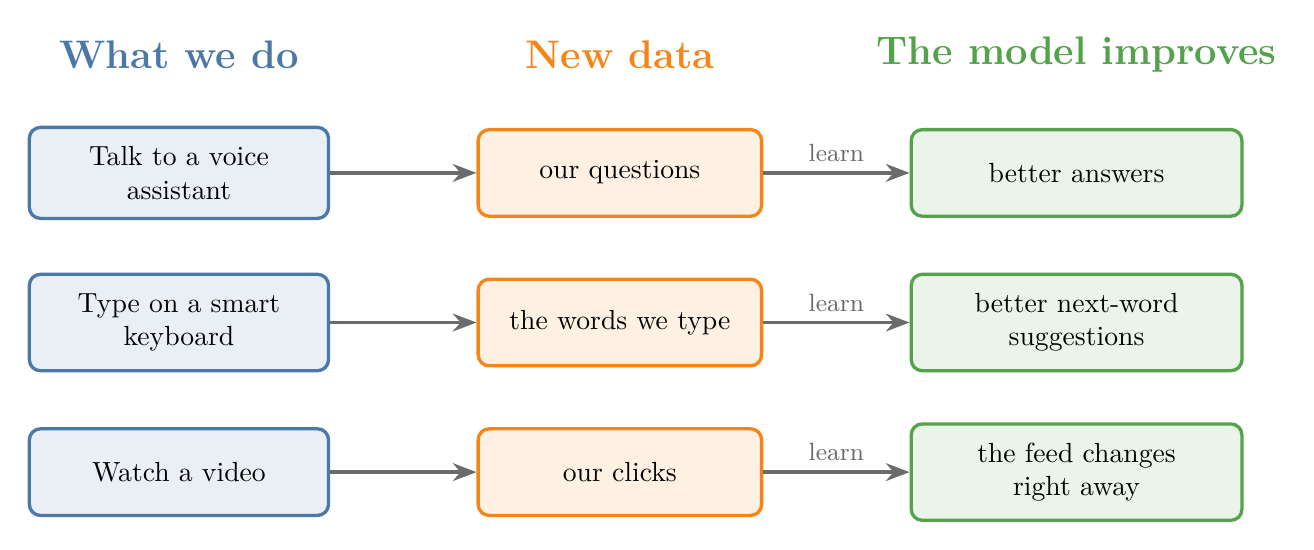
\begin{tikzpicture}
  \node[title, text=cblue] at (0,1.5) {What we do};
  \node[title, text=corange] at (5.6,1.5) {New data};
  \node[title, text=cgreen] at (11.4,1.5) {The model improves};
  \foreach \n/\y/\a/\b/\c in {1/0/{Talk to a voice\\assistant}/{our questions}/{better answers},
                              2/-1.9/{Type on a smart\\keyboard}/{the words we type}/{better next-word\\suggestions},
                              3/-3.8/{Watch a video}/{our clicks}/{the feed changes\\right away}}
    { \node[box=cblue, minimum width=3.8cm] (a\n) at (0,\y) {\a};
      \node[box=corange, minimum width=3.6cm] (b\n) at (5.6,\y) {\b};
      \node[box=cgreen, minimum width=4.2cm] (c\n) at (11.4,\y) {\c};
      \draw[arrow] (a\n) -- (b\n); \draw[arrow] (b\n) -- node[note, above] {learn} (c\n); }
\end{tikzpicture}
\end{document}
